\documentclass[11pt, reqno]{amsart}
\usepackage[margin=1in]{geometry}
\geometry{letterpaper}
%\geometry{landscape} % Activate for for rotated page geometry
\usepackage[parfill]{parskip} % Activate to begin paragraphs with an
% empty line rather than an indent
\usepackage{amsfonts, amscd, amssymb, amsthm, amsmath}
\usepackage{mathtools} %xmapsto etc
\usepackage{pdfsync} %leaves makers for tex searching
\usepackage{enumerate}

%%% Color %%%---------------------------------------------------------
\usepackage{color}
\usepackage[dvipsnames]{xcolor}
\definecolor{dred}{HTML}{C30101}
\definecolor{dorange}{rgb}{.9,.3,0}
\definecolor{dgrey}{rgb}{.4,.4,.4}
\definecolor{plumb}{HTML}{8105C1}
\definecolor{pumpkin}{HTML}{E47604}
\definecolor{rose}{HTML}{C10091}
\definecolor{dgreen}{HTML}{25A75B}
\definecolor{dblue}{HTML}{0066FF}
\definecolor{cornflower}{HTML}{3256C3}
\definecolor{viridian}{HTML}{099A97}
\definecolor{alert}{HTML}{3256C3}

\newcommand\plumb[1]{{\color{plumb}#1}}
\newcommand\cornfl[1]{{\color{cornflower}#1}}
\newcommand\dgreen[1]{{\color{dgreen}#1}}
\newcommand\viridian[1]{{\color{viridian}#1}}
\newcommand\dblue[1]{{\color{dblue}#1}}
\newcommand\dred[1]{{\color{dred}#1}}
\newcommand\gray[1]{{\color{black!40}#1}}
\newcommand\black[1]{{\color{black}#1}}
\newcommand\pumpk[1]{{\color{pumpkin}#1}}
\newcommand\rose[1]{{\color{rose}#1}}

\newcommand{\NOTE}[1]{{\color{cornflower}#1}}
\newcommand{\alert}[1]{{\color{alert}#1}}
\newcommand{\Alert}[1]{\emph{\color{alert}#1}}

\usepackage{hyperref} %[pdftex,bookmarks]
\hypersetup{
  colorlinks=true,
  linkcolor=viridian,
  filecolor=viridian,
  citecolor=viridian,
  urlcolor=viridian,
  pdfpagemode=FullScreen,
}

%%% Theorems %%%---------------------------------------------------------
\theoremstyle{plain}
\newtheorem*{thm}{Theorem}
\newtheorem*{lemma}{Lemma}
\newtheorem*{prop}{Proposition}
\newtheorem*{cor}{Corollary}
\theoremstyle{definition}
\newtheorem*{defn}{Definition}
\newtheorem*{remark}{Remark}

%%% Environments %%%---------------------------------------------------------
\newenvironment{pf}{\color{black}\medskip
\paragraph*{\emph{Proof}.}}{\hfill \qedsymbol \medskip }
\newenvironment{ans}{\medskip \color{black}
\paragraph*{\emph{Answer}.}}{\hfill \break $~\!\!$ \dotfill \medskip }
\newenvironment{sketch}{\medskip \paragraph*{\emph{Proof sketch}.}}{ \medskip }
\newenvironment{summary}{\medskip \paragraph*{\emph{Summary}.}}{
\hfill \break \rule{1.5cm}{0.4pt} \medskip }
\newcommand\Ans[1]{$ $\hfill {\color{black}\emph{Answer:} {#1}}}
\newcommand{\Hint}[1]{{\small [\emph{Hint:} {#1}]}}

%%% Pictures %%%---------------------------------------------------------
%%% If you need to draw pictures, tikzpicture is one good option.
% Here are some basic things I always use:
\usepackage{tikz}
\usetikzlibrary{scopes}
\usetikzlibrary{automata}
\usetikzlibrary{positioning}
\usepgflibrary{shapes}
\tikzstyle{V}=[draw, fill =black, circle, inner sep=0pt, minimum size=2pt]
\tikzstyle{bV}=[draw, fill =black, circle, inner sep=0pt, minimum size=4pt]
\tikzstyle{over}=[draw=white,double=black,line width=3pt]
\tikzstyle{C}=[draw, thick, fill =white, circle, inner sep=0pt,
minimum size=6pt]

\newcommand\TikZ[1]{
  \begin{matrix}
    \begin{tikzpicture}#1
    \end{tikzpicture}
\end{matrix}}

\newcounter{r}
\newcommand\Part[1]{
  \setcounter{r}{1}
  \foreach \x in {#1}{
    {\ifnum\value{r}=1
      \draw (0,\value{r}-1)--(\x,\value{r}-1);
    \fi}
    \draw (0,\value{r}) to (\x,\value{r});
    \foreach \y in {0, ..., \x} {\draw (\y,\value{r})--(\y,\value{r}-1);}
    \addtocounter{r}{1}
}}
\def\PartUNIT{.175}
%Self-contained tikz images for \Part above.
\newcommand{\PART}[1]{
  \begin{matrix}
    \begin{tikzpicture}[xscale=\PartUNIT, yscale=-\PartUNIT]
      \Part{#1}
    \end{tikzpicture}
  \end{matrix}
}

\def\FOUR{4}\def\ONE{1}\def\FIVE{5}\def\EIGHT{8}\def\THREE{3}\def\TWO{2}\def\SIX{6}\def\SEVEN{7}

%%% Alphabets %%%---------------------------------------------------------
%%% Some shortcuts for my commonly used special alphabets and characters.
\def\cA{\mathcal{A}}\def\cB{\mathcal{B}}\def\cC{\mathcal{C}}\def\cD{\mathcal{D}}\def\cE{\mathcal{E}}\def\cF{\mathcal{F}}\def\cG{\mathcal{G}}\def\cH{\mathcal{H}}\def\cI{\mathcal{I}}\def\cJ{\mathcal{J}}\def\cK{\mathcal{K}}\def\cL{\mathcal{L}}\def\cM{\mathcal{M}}\def\cN{\mathcal{N}}\def\cO{\mathcal{O}}\def\cP{\mathcal{P}}\def\cQ{\mathcal{Q}}\def\cR{\mathcal{R}}\def\cS{\mathcal{S}}\def\cT{\mathcal{T}}\def\cU{\mathcal{U}}\def\cV{\mathcal{V}}\def\cW{\mathcal{W}}\def\cX{\mathcal{X}}\def\cY{\mathcal{Y}}\def\cZ{\mathcal{Z}}

\def\AA{\mathbb{A}} \def\BB{\mathbb{B}} \def\CC{\mathbb{C}} \def\DD{\mathbb{D}}
\def\EE{\mathbb{E}} \def\FF{\mathbb{F}} \def\GG{\mathbb{G}} \def\HH{\mathbb{H}}
\def\II{\mathbb{I}} \def\JJ{\mathbb{J}} \def\KK{\mathbb{K}} \def\LL{\mathbb{L}}
\def\MM{\mathbb{M}} \def\NN{\mathbb{N}} \def\OO{\mathbb{O}} \def\PP{\mathbb{P}}
\def\QQ{\mathbb{Q}} \def\RR{\mathbb{R}} \def\SS{\mathbb{S}} \def\TT{\mathbb{T}}
\def\UU{\mathbb{U}} \def\VV{\mathbb{V}} \def\WW{\mathbb{W}} \def\XX{\mathbb{X}}
\def\YY{\mathbb{Y}} \def\ZZ{\mathbb{Z}}

\def\fa{\mathfrak{a}} \def\fb{\mathfrak{b}} \def\fc{\mathfrak{c}}
\def\fd{\mathfrak{d}} \def\fe{\mathfrak{e}} \def\ff{\mathfrak{f}}
\def\fg{\mathfrak{g}} \def\fh{\mathfrak{h}} \def\fj{\mathfrak{j}}
\def\fk{\mathfrak{k}} \def\fl{\mathfrak{l}} \def\fm{\mathfrak{m}}
\def\fn{\mathfrak{n}} \def\fo{\mathfrak{o}} \def\fp{\mathfrak{p}}
\def\fq{\mathfrak{q}} \def\fr{\mathfrak{r}} \def\fs{\mathfrak{s}}
\def\ft{\mathfrak{t}} \def\fu{\mathfrak{u}} \def\fv{\mathfrak{v}}
\def\fw{\mathfrak{w}} \def\fx{\mathfrak{x}} \def\fy{\mathfrak{y}}
\def\fz{\mathfrak{z}} \def\fgl{\mathfrak{gl}}  \def\fsl{\mathfrak{sl}}
\def\fso{\mathfrak{so}}  \def\fsp{\mathfrak{sp}}  \def\GL{\mathrm{GL}}
\def\SL{\mathrm{SL}}  \def\SP{\mathrm{SL}}\def\OG{\mathrm{O}}

\def\aa{\mathbf{a}} \def\bb{\mathbf{b}} \def\cc{\mathbf{c}} \def\dd{\mathbf{d}}
\def\ee{\mathbf{e}} \def\ff{\mathbf{f}}
%\def\gg{\mathbf{g}}
\def\hh{\mathbf{h}} \def\ii{\mathbf{i}} \def\jj{\mathbf{j}} \def\kk{\mathbf{k}}
%\def\ll{\mathbf{l}}
\def\mm{\mathbf{m}} \def\nn{\mathbf{n}} \def\oo{\mathbf{o}} \def\pp{\mathbf{p}}
\def\qq{\mathbf{q}} \def\rr{\mathbf{r}} \def\ss{\mathbf{s}} \def\tt{\mathbf{t}}
\def\uu{\mathbf{u}} \def\vv{\mathbf{v}} \def\ww{\mathbf{w}} \def\xx{\mathbf{x}}
\def\yy{\mathbf{y}} \def\zz{\mathbf{z}} \def\zzero{\mathbf{0}}

\def\<{\langle} \def\>{\rangle}
\def\Aut{\mathrm{Aut}}
\def\ch{ \stackrel}
\def\col{\mathrm{col}}
\def\dim{\mathrm{dim}}
\def\End{\mathrm{End}}
\def\ev{\mathrm{ev}}
\def\f{\varphi}
\def\gcd{\mathrm{gcd}}
\def\half{\hbox{$\frac12$}}
\def\Hom{\mathrm{Hom}}
\def\img{\mathrm{img}}
\def\id{\mathrm{id}}
\def\Inn{\mathrm{Inn}}
\def\lcm{\mathrm{lcm}}
\def\normeq{\trianglelefteq}
%\def\ch{ \stackrel{\mathrm{ch}}{\trianglelefteq}}
%\def\normeq{\trianglelefteq}
\def\nul{\mathrm{nullity}}
\def\row{\mathrm{row}}
\def\rk{\mathrm{rank}}
\def\sgn{\mathrm{sgn}}
\def\sp{\mathrm{span}}
\def\supp{\mathrm{supp}}
\def\Syl{\mathrm{Syl}}
\def\tr{\mathrm{tr}}
\def\vep{\varepsilon}

\usepackage{mathabx}
\def\acts{\lefttorightarrow} %group action

%\usepackage{mathtools}
\usepackage{wasysym}

\def\ol{\overline}
\newcommand{\Mod}[1]{\ (\mathrm{mod}\ #1)}

\def\Hfill{$ $\hfill}

% Arrows:
\newcommand\xdhrightarrow[2][]{%
  \mathrel{\ooalign{$\xrightarrow[#1\mkern4mu]{#2\mkern4mu}$\cr%
  \hidewidth$\rightarrow\mkern4mu$}}
}
%\newcommand\dhrightarrow{%
% \mathrel{\ooalign{$\rightarrow$\cr%
% $\mkern3.5mu\rightarrow$}}
%}
\def\dhrightarrow{\twoheadrightarrow}
\def\dhleftarrow{\twoheadleftarrow}
\def\tab{\hspace{10pt}}

% Arrays:
\newcommand\Pmatrix[1]{
  \begin{pmatrix}#1
\end{pmatrix}}
\newcommand\smatrix[1]{\text{\small$
    \begin{pmatrix}#1
\end{pmatrix}$}}
\newcommand\fmatrix[1]{\text{\footnotesize$
    \begin{pmatrix}#1
\end{pmatrix}$}}
\newcommand\tmatrix[1]{\text{\tiny$
    \begin{pmatrix}#1
\end{pmatrix}$}}

\makeatletter
\newcommand{\chareq}{%
  \mathrel{\mathpalette\chRAW\relax}%
}

\newcommand{\chRAW}[2]{%
  \sbox\z@{$#1\LHD$}%
  \sbox\tw@{$#1\leqslant$}%
  \dimen@=\ht\tw@
  \advance\dimen@-\ht\z@
  \advance\dimen@ .3pt
  \ifx#1\displaystyle
  \advance\dimen@ .2pt
  \else
  \ifx#1\textstyle
  \advance\dimen@ .2pt
  \fi
  \fi
  \ooalign{\raisebox{\dimen@}{$\m@th#1\LHD$}\cr$\m@th#1\leqslant$\cr}%
}
\makeatother

%%%%%%%%%%%%%%%%%%%%%%%%%%%%%%
%%%%%%%%%%%%%%%%%%%%%%%%%%%%%%

\def\HW{7}
\def\DUE{April 8th, 2025 by 10:30am}

\title[Homework \HW]{Homework \HW \\
  Math 332, \S S01/02\\
\small Due: \DUE}
\author{}
%\date{}   % Activate to display a given date or no date

\begin{document}
% \maketitle %%% COMMENT THIS OUT and UNCOMMENT the following to give
% yourself a good assignment header:
\begin{flushleft}
  Bram Schuijff\\
  CSCI 387, \S S01/02\\
  Homework \HW\\
  \DUE
\end{flushleft}

\begin{enumerate}
  \item[1.] In order to formulate this problem as a language, we can phrase it
    in the following way:
    \begin{align*}
      L =~&\{\langle G, K\rangle~|~\text{For $G = (V, E)$ a graph with
        $K\subseteq V$,}\\
        &\text{there exists a set of vertices $M\subseteq V\setminus K$
        such that for each $k\in K$,}\\
        &\text{$k$ is adjacent to exactly $n(k)$ vertices in $M$ where
      $n(k)$ is the label of $k$}\}
    \end{align*}
    To demonstrate that $L$ is $\NN\PP$-complete, we must first show that $L$
    is in $\NN\PP$. To do so, we can construct a polynomial-time verifier $D$
    for $L$. When given an input $\langle G, K, w\rangle$, $D$ can check first
    that $K, M\subseteq V$ and furthermore that $K\cap M = \emptyset$.
    Traversing the vertex set of $M$ and $K$ is certainly polynomial time and
    then comparing them against each other is $O(|V|^2)$ time. Therefore, this
    step can be done in polynomial time. To verify that an assignment is valid,
    we can simply iterate through each $k\in K$, check its adjacency list, and
    then see if there are exactly $n(k)$ vertices adjacent to $k$ that are in
    $M$. If there are not, reject. If we have not rejected by the time we have
    iterated through each $k$ in $K$, accept. This can be done in $O(|V|^2)$
    time because that is the most amount of time it can take to check all of
    the adjacent vertices of all vertices in $G$. Therefore, $D$ is polynomial
    time in the size of $\langle G, K\rangle$.

    To check that $D$ verifies $L$, we see first that any witness that $D$ will
    accept necessarily has $M$ and $K$ being disjoint. Any valid witness will
    have this property because if there exists an $e\in M\cap K$, then a mine
    would have been revealed and the game would be over. Then, we simply check
    that every revealed node has exactly as many mines adjacent to it as its
    value says it does. If it does not, then the graph is necessarily
    inconsistent because there exists a revealed node whose value is more or
    less than the number of mines it is adjacent to and we reject. If all
    revealed nodes have precisely the number of mines adjacent to them as their
    s value indicates, then the graph is consistent by definition. Therefore,
    we accept. Thus, $D$ decides $L$ and therefore $L$ is in $\NN\PP$.

    % If our binary expression has a satisfying assignment -> there exists a
    % consistent Minesweeper assignment. Given a binary expression X, turn it
    % into a graph and a revealed set K such that solving the graph and the
    % revealed set would also solve the binary expression

    % Variable gadget: it cannot be that both X and not X are True. Clause
    % gadget: at least one variable from each clause must be True. What is our
    % truth value here? What are we taking to be True? Clearly our variables
    % correspond to the vertices of G but is placing a node into the mine set
    % considered setting that variable as True? Is having one of X and not X
    % being in the mine set and the other being in the revealed set a way to
    % encode our variable gadget?
    To demonstrate that $L$ is $\NN\PP$-complete, we can perform a reduction
    from 3SAT. Given a 3-cnf boolean expression $X$, we are attempting
    to produce a graph and revealed vertex set $G, K$ such that finding whether
    or not $G, K$ is in $L$ would prove the satisfiability of $X$.

    We can start by recognizing what our truth value is supposed to be. For my
    construction, I am going to assign each literal to exactly one unrevealed
    vertex in $G$. Then, a variable being marked as True is associated with
    having a mine marker placed on that variable's associated vertex.

    We can start by constructing a variable gadget. We want it to be that for a
    variable $x$, either $x$ or $\bar{x}$ is True. Therefore, only $x$ or
    $\bar{x}$ can have a mine placed on top of it. Therefore, we create a setup
    whereby $x$ and $\bar{x}$ are adjacent to each other and they are both
    adjcaent to a revealed vertex whose value is $1$. Thus, if there is a
    satisfying assignment, it cannot be that both $x$ and $\bar{x}$'s vertices
    have mines. A visual demonstration follows:
    \begin{center}
      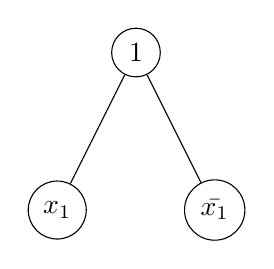
\begin{tikzpicture}
        \node [circle, draw] (1) at (0, 0) {$1$};
        \node [circle, draw] (x_1) at (-1, -2) {$x_1$};
        \node [circle, draw] (not x_1) at (1, -2) {$\bar{x_1}$};
        \draw (1)--(x_1);
        \draw (1)--(not x_1);
      \end{tikzpicture}
    \end{center}
    Then, to construct a clause gadget, we want it to be that for each clause,
    at least one of the variable's associated vertices has a mine. To do so, we
    can construct a gadget whereby if $3$ variables are in the same clause,
    they are all connected to a vertex labelled $3$. That vertex labeled $3$ is
    additionally connected to $2$ other unrevealed vertices not associated with
    any variable. For instance, in the clause $x\lor y\lor z$, we would produce
    the following component:
    \begin{center}
      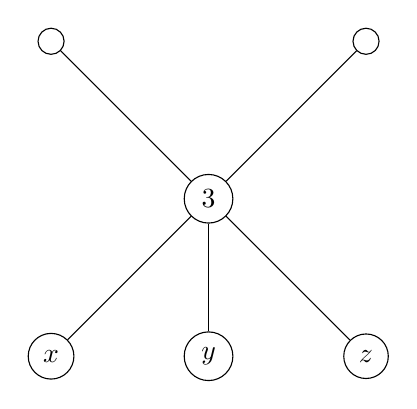
\begin{tikzpicture}
        \node [circle, draw] (x) at (-2, -2) {$x$};
        \node [circle, draw] (y) at (0, -2) {$y$};
        \node [circle, draw] (z) at (2, -2) {$z$};
        \node [circle, draw] (3) at (0, 0) {$3$};
        \node [circle, draw] (b1) at (2, 2) {};
        \node [circle, draw] (b2) at (-2, 2) {};
        \draw (x)--(3);
        \draw (z)--(3);
        \draw (y)--(3);
        \draw (3)--(b1);
        \draw (3)--(b2);
      \end{tikzpicture}
    \end{center}
    This guarantees that at least one of $x, y, z$ contains a mine because $3$
    has already been revealed and therefore cannot contain a mine itself. In
    order for this graph to be consistent, then because there are only $2$
    other unrevealed nodes connected to $3$, one of $x, y, z$ has to contain a
    mine. If a clause only has two variables (for instance $x\lor x \lor y$)
    then we simply get rid of the $z$ and connect the vertex labelled $3$ to
    $x$ and $y$. Meanwhile, if a clause consists of only one variable like with
    $x\lor x\lor x$, then we simply connect the $3$ to $x$ and the two other
    unlabelled, unrevealed vertices.

    To show that this construction is actually a reduction, we find that the
    construction is inherently consistent---either $x$ or $\bar{x}$ contains a
    mine---and that each clause must contain at least one mine. Therefore, if
    we let our mines represent True, we have that demonstrating $G, K$ is
    consistent is equivalent to showing that $X$ has a satisfying assignment.

    In this construction, we find that because each variable $x$ has a vertex
    in $K$ associated with its variable gadget and each clause has $3$ vertices
    associated with its clause gadget, we get $|K| = n\cdot m$ if $m$ is the
    number of clauses and $n$ is the number of variables. Then, $|V| = 2n +
    |K|$. These are both polynomial in the length of our boolean expression.
    Because $|E| \in O(|V|^2)$, we then have that we can also construct all of
    our edges in polynomial time. Therefore, this reduction is polynomial time.

    Therefore, because $L\in \NN\PP$ and there exists a polynomial-time
    reduction from 3SAT to $L$ and 3SAT is $\NN\PP$-complete, we have that $L$
    is $\NN\PP$-complete.

  \item[2.] Because PSPACE = NPSPACE by Savitch's Theorem, if we can demonstrate
    that there exists a nondeterministic polynomial space Turing machine which
    decides GOMOKU, we are done. Let $D$ be the following nondeterministic
    Turing machine:
    \begin{enumerate}[1.]
      \item On input $\langle C\rangle$:
      \item \tab If $C$ contains $5$ contiguous red pieces, accept.
      \item \tab If $C$ contains $5$ contiguous blue pieces, reject.
      \item \tab If every square but $1$ on $C$ is covered:
      \item \tab\tab If it is the blue player's turn, reject.
      \item \tab\tab If
        there are not $4$ red pieces adjacent to the empty square, reject.
      \item \tab If it is not the red player's turn, jump to step 9.
      \item \tab Nondeterministically select an unmarked space and place a red
        token there.
      \item \tab For each available space $c_{i, j}$ on the board:
      \item \tab\tab Place a blue piece at $c_{i, j}$ and call this
        configuration $C[i,j]$.
      \item \tab\tab Spawn a child process $D(\langle C[i,j]\rangle)$.
      \item \tab\tab If $D(\langle C[i, j]\rangle)$ rejects, reject. Otherwise,
        continue.
      \item \tab If we have not yet rejected, accept.
    \end{enumerate}
    We know that $D$ decides GOMOKU because given a configuration $C$, we can
    nondeterministically select the best move for red and then attempt every
    single response that blue could produce. If blue has a move that allows
    them to win or force a tie as we check for in steps 3 to 6, we reject
    because red cannot force a win from the configuration $C$. However, if blue
    attempts every single response and still cannot win or force a tie, then we
    accept because red can force a win no matter what blue attempts. We have
    the base case in step 2 where if a configuration has 5 contiguous red
    pieces, then red wins from that configuration.

    We know that $D\in\text{PSPACE}$ because each child process occupies space
    in $O(n^2)$ where $n$ is the length of one side of the board. Furthermore,
    we have a recursive depth in $O(n^2)$ because we fork at most to the depth
    that it takes to fill the board; the number of child processes spawned at
    any point is irrelevant. Therefore, $D$ occupies space in $O(n^4)$ which is
    polynomial. Therefore, $\text{GOMOKU}\in\text{PSPACE}$.

  \item[3.] To demonstrate that PSPACE is closed under the star operation, let
    $L$ be a language in PSPACE. Now, we want to show that
    $L^*\in\text{PSPACE}$. Because $L\in\text{PSPACE}$, there exists a
    polynomial space decider $D$ for $L$. We can now construct a polynomial
    space decider $D^*$ for $L^*$ as follows:
    \begin{enumerate}[1.]
      \item On input $\langle w\rangle$:
      \item \tab If $w = \epsilon$, accept.
      \item \tab Let $p = 0$.
      \item \tab Loop:
      \item \tab\tab Nondeterministically set $d$ such that $p < d \leq |w|$.
      \item \tab\tab Run $D(\langle w[p, d]\rangle)$ with Pythonic string
        slicing. If it rejects, reject.
      \item \tab\tab Set $p = d$.
      \item \tab\tab If $d = |w|$, accept.
    \end{enumerate}
    This is a decider for $L^*$ because for any string $w\in L^*$, we have that
    $w = w_1w_2w_3...w_n$ where $w_i\in L$ for all $i$ or that $w = \epsilon$.
    If $w = \epsilon$, it is vacuously in $L^*$ by the nature of the star
    operation. Otherwise, if we can iterate through and find the division
    points between the slices that make up $w$, we are done because we can just
    run the decider for $L$ on each slice and $D^*$ will accept $w$. Meanwhile,
    if no such division exists, then there is exists at least one substring
    $w_j$ in $w$ such that $w_j\notin L$, at which point $D$ will reject $w_j$
    and therefore $D^*$ will reject $w$. Thus, $D^*$ decides $L^*$.

    To show that $D^*$ is in PSPACE, we will first show that $D^*$ is in
    NPSPACE. Steps 2 and 3 can clearly be done in polynomial space because $L$
    is in PSPACE. Meanwhile, steps 4, 6 and 8 are space in proportion to
    $\langle w\rangle$. Then, step 7 is polynomial space because $L$ is in
    PSPACE. Finally, our end condition occupies constant space. Therefore,
    $D^*$ occupies polynomial space and $L^*\in\text{NPSPACE}$. By Savitch's
    theorem, we also have that $L^*\in\text{PSPACE}$ and therefore PSPACE is
    closed under the star operation.
\end{enumerate}

\end{document}
